\documentclass{beamer}
\usepackage{beamerthemesplit}

%Definieren uns farbigen Quellcode
\usepackage{color}
\definecolor{dkgreen}{rgb}{0,0.6,0}
\definecolor{gray}{rgb}{0.5,0.5,0.5}
\definecolor{mauve}{rgb}{0.58,0,0.82}
 
%Damit wir Quellcode nutzen können.
\usepackage{listings}
\lstset{numbers=left,
	numberstyle=\tiny,
	numbersep=5pt,
	breaklines=true,
	showstringspaces=false,
	frame=l ,
	xleftmargin=15pt,
	xrightmargin=15pt,
	basicstyle=\ttfamily\scriptsize,
	stepnumber=1,
	keywordstyle=\color{blue},          % keyword style
  	commentstyle=\color{dkgreen},       % comment style
  	stringstyle=\color{mauve}         % string literal style
}
%Sprache Festelegen
\lstset{language=C++}

\begin{document}
\title{Infinite Impulse Response Filters} 
\author{Judith Massa, Patrick Esser}
\date{\today} 

\frame{\titlepage} 

\frame{\frametitle{Overview}\tableofcontents} 

\section{Motivation} 
\frame{\frametitle{Ilastik}
\begin{figure}
\begin{tabular}{c}
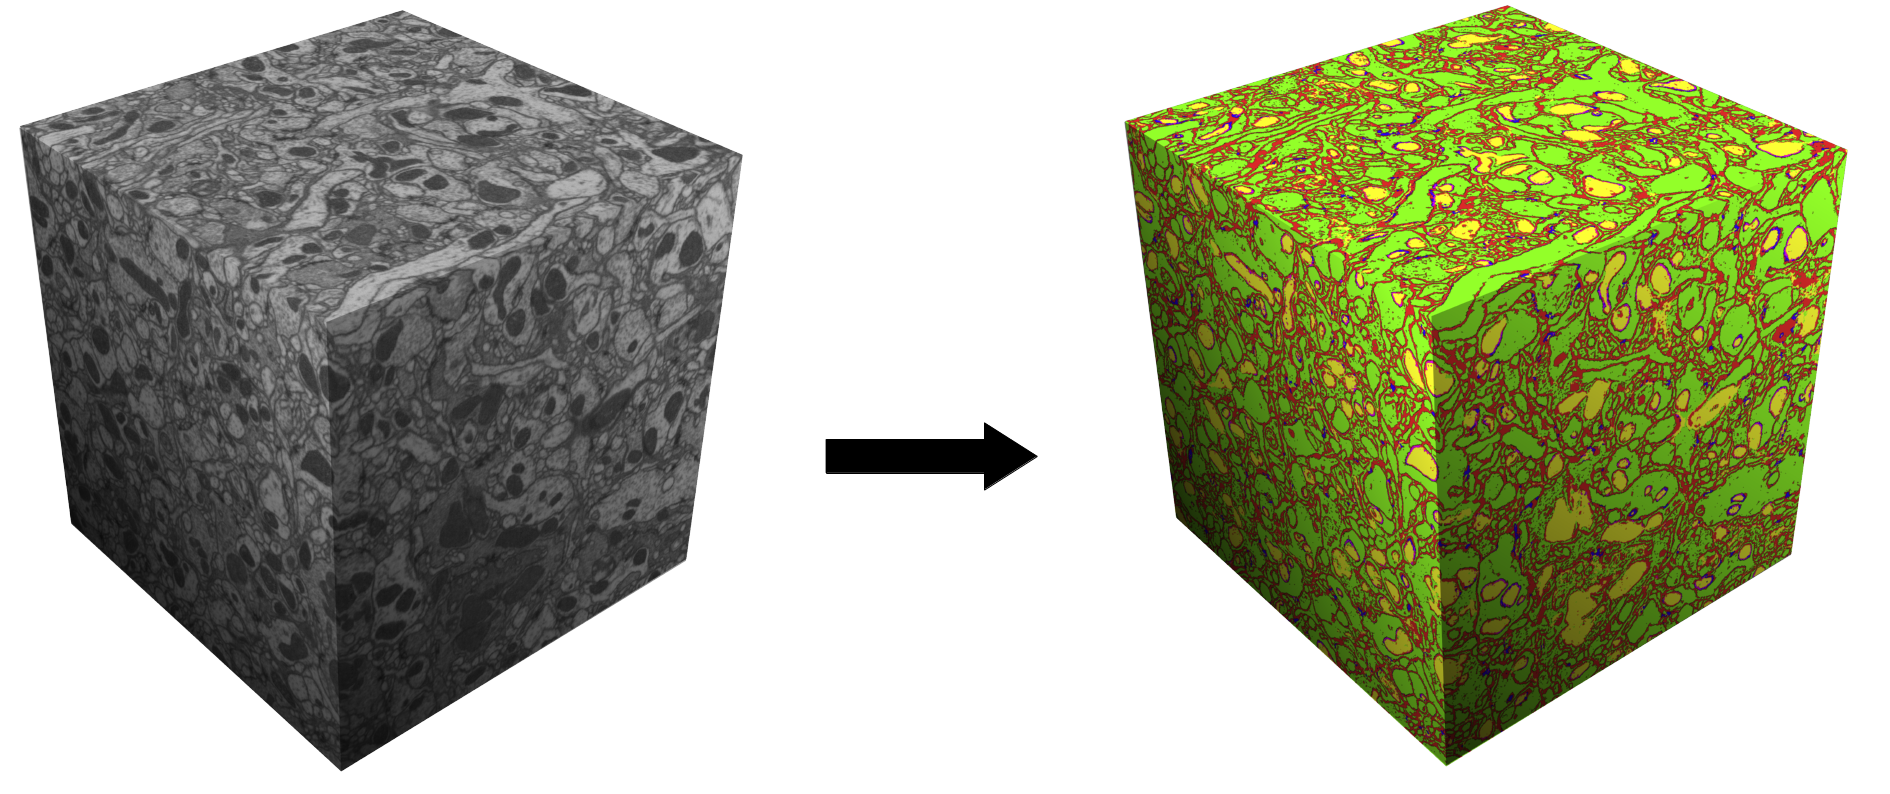
\includegraphics[scale=0.1]{imgs/cubes_combined.jpg}
\end{tabular}
\end{figure}
\begin{itemize}
  \item Ilastik: toolkit for interactive image classification and segmentation
  \item Algorithms rely on precomputed features of the image
\end{itemize}
\begin{figure}
\centering
\begin{tabular}{ccc}
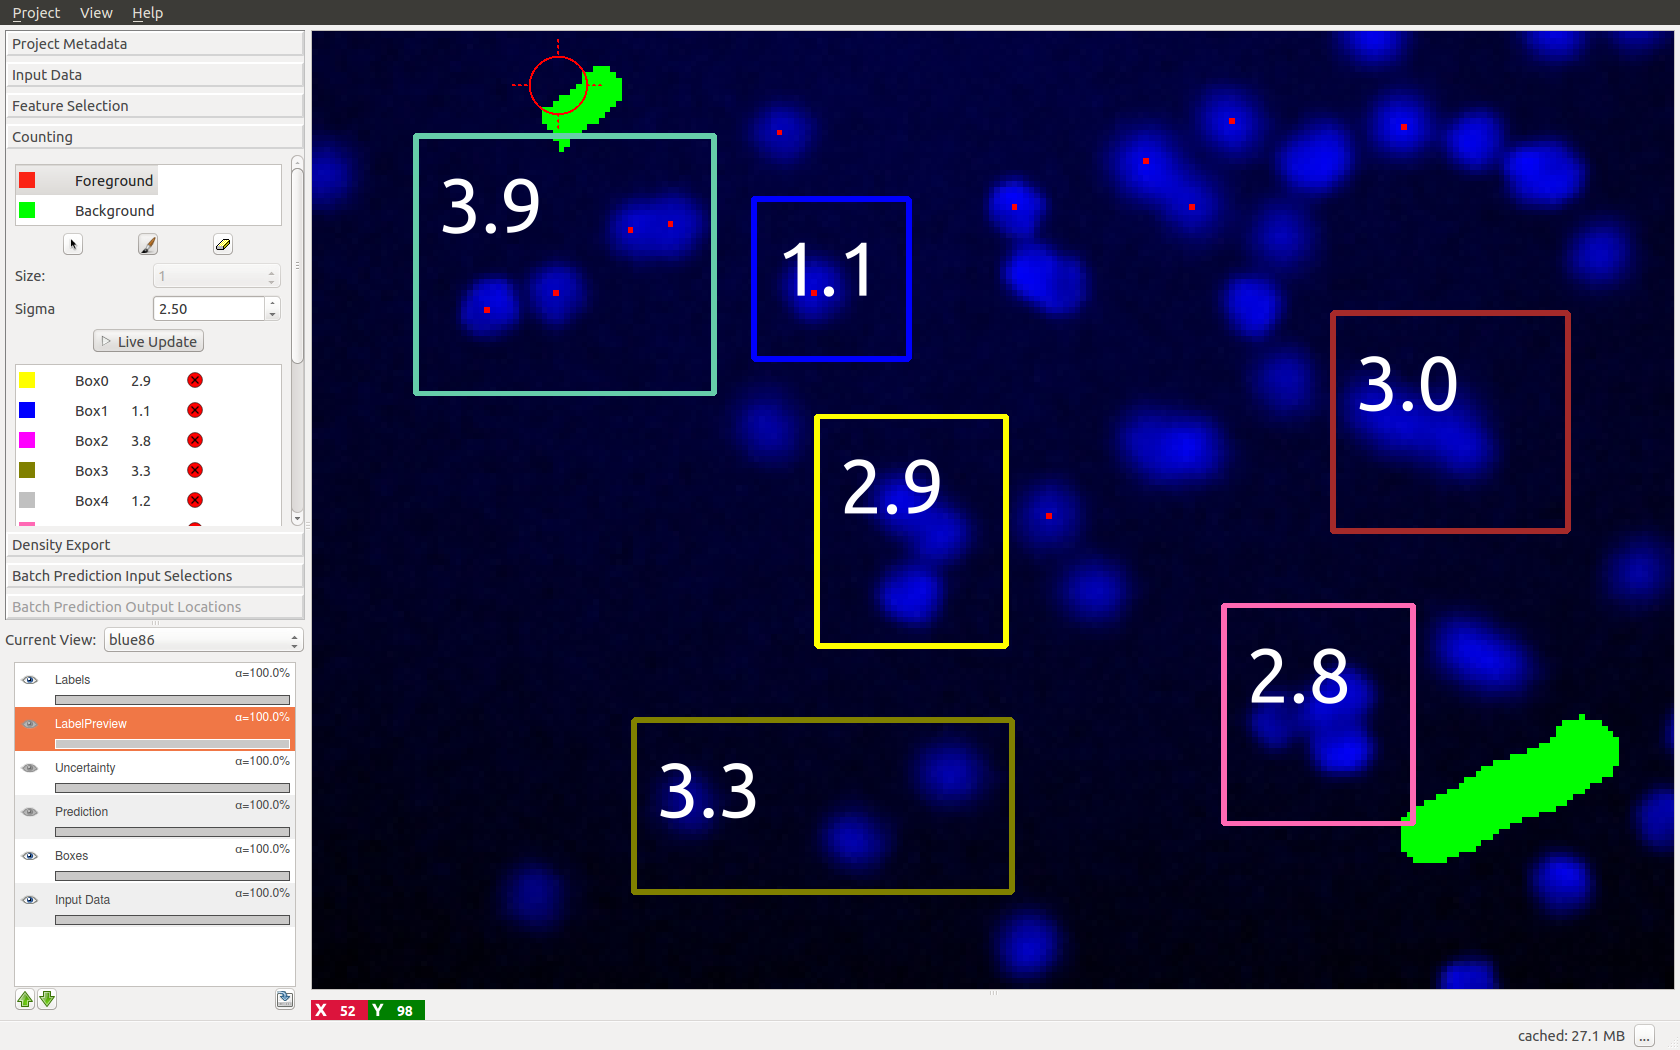
\includegraphics[scale=0.05]{imgs/ilastik1.png}\quad &
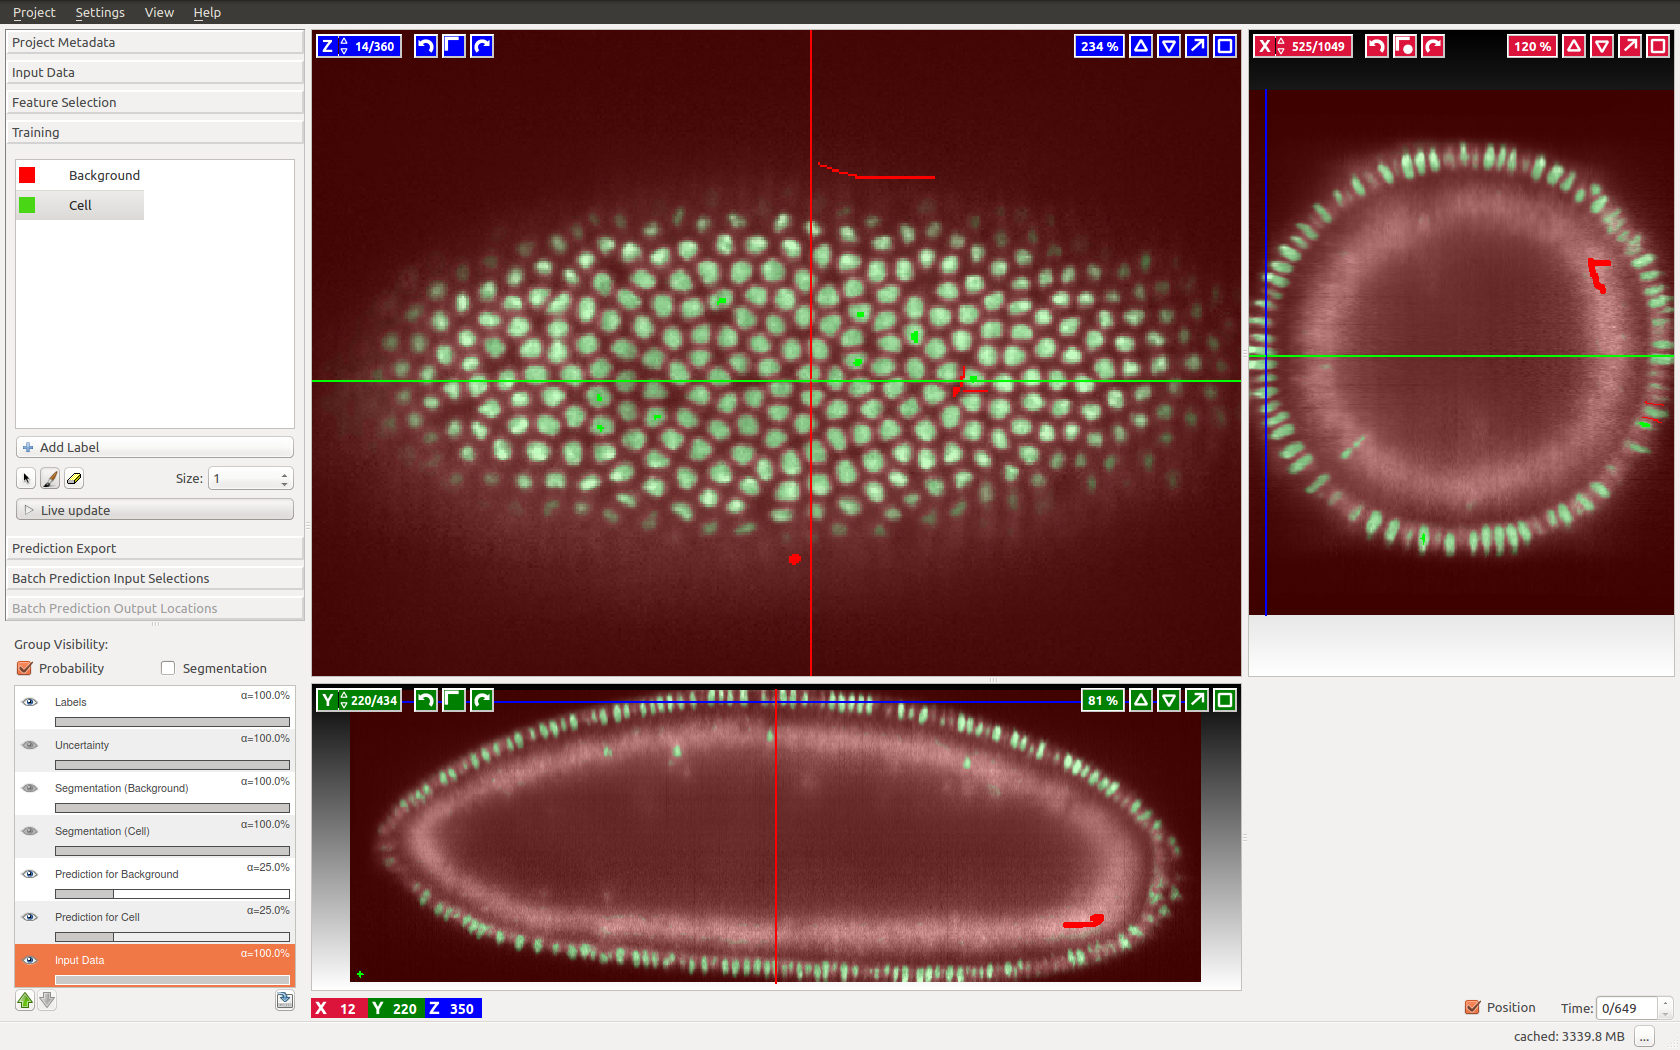
\includegraphics[scale=0.05]{imgs/ilastik2.png}\quad &
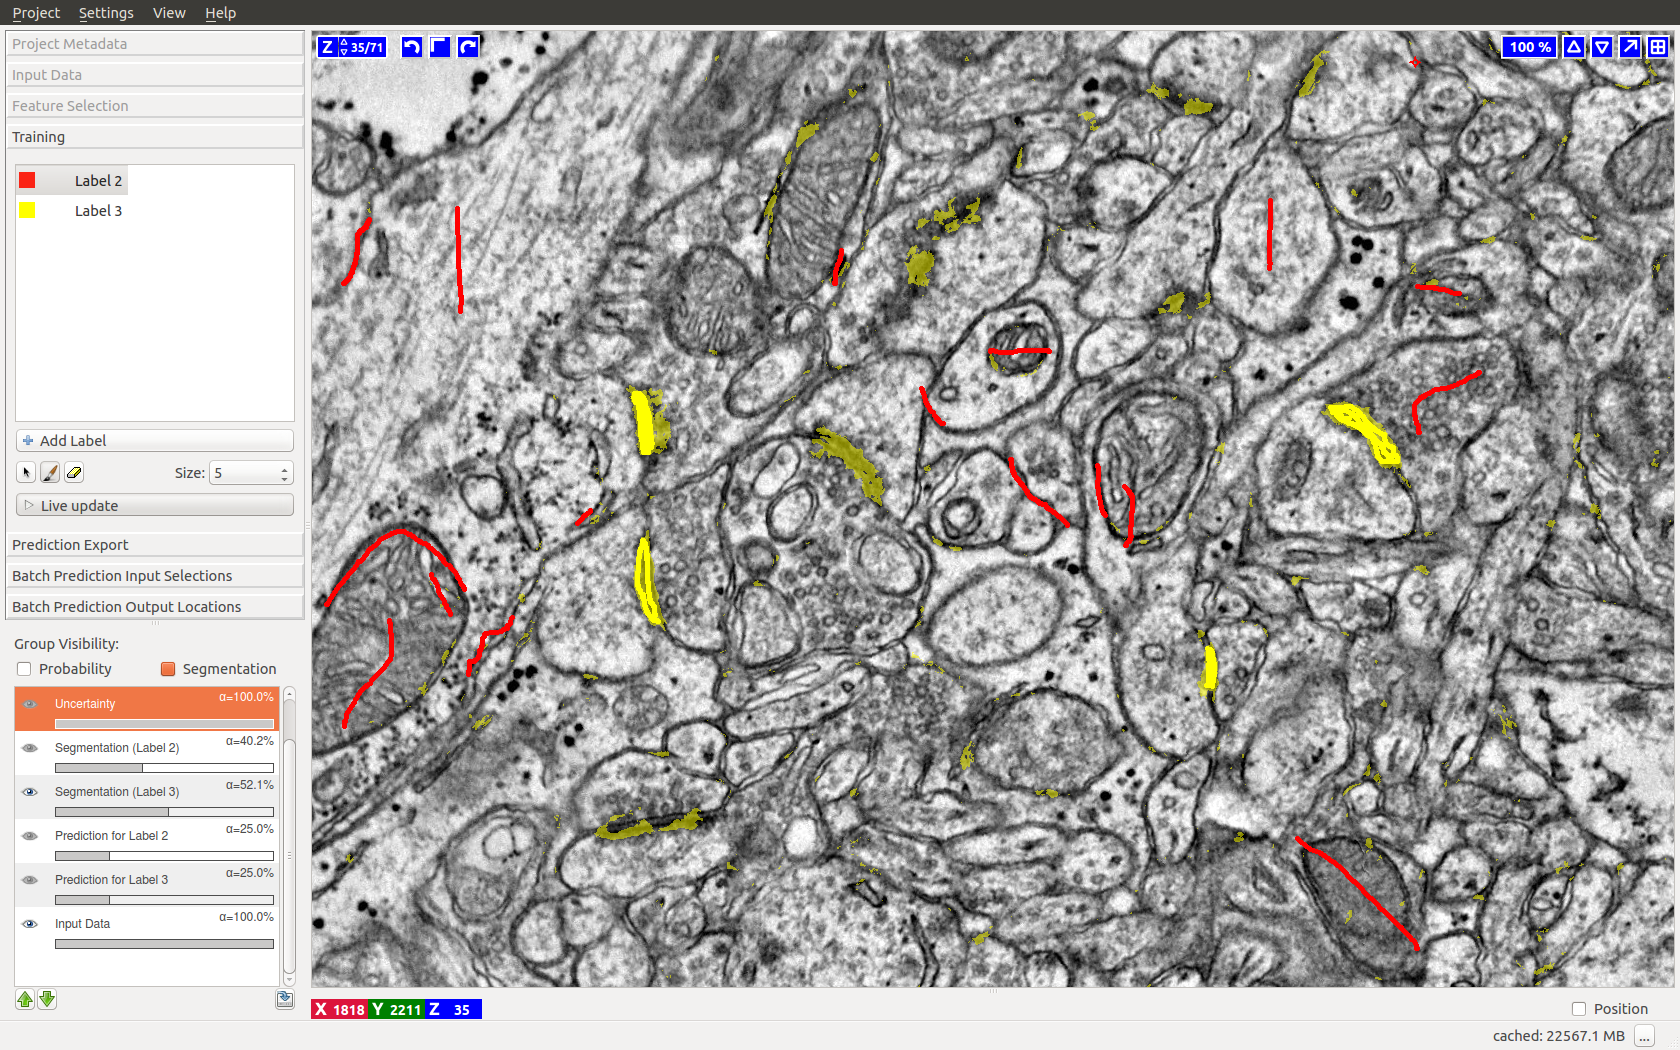
\includegraphics[scale=0.07]{imgs/ilastik3.png} 
\end{tabular}
\end{figure}
}

\frame{\frametitle{Tracking}
Example:
\begin{itemize}
  \item Project supervisor Sven Peter is working on object tracking \\
        $\to$ Requires classification scale space and edge detection
\end{itemize}
\begin{figure}
\centering
\begin{tabular}{cc}
\includegraphics[scale=0.08]{imgs/tracking1.png}\quad &
\includegraphics[scale=0.08]{imgs/tracking2.png} 
\end{tabular}
\end{figure}
}

%\frame{\frametitle{Image Features} 
%\begin{itemize}
  %\item Edges
  %\item Corners
  %\item Scale-space representation
%\end{itemize}
%}

\frame{\frametitle{Gaussian Filtering}
Convolution: 
$$(f*g)(x) := \int_{\mathbb{R}^n} f(\tau)g(x-\tau)\mathrm{d}\tau$$
\begin{itemize}
  \item discrete: $(f*g)[n]=\sum_{m=-\infty}^\infty f[n-m]\, g[m]$
  \item $f\ldots$ image
  \item $g\ldots$ signal, e.g. Gaussian
\end{itemize}

Gaussian:
\begin{itemize}
  \item $g=\frac{1}{\sqrt{2\sigma^2\pi}}e^{-{\frac {(x-\mu)^{2}}{2\sigma^{2}}}}$
  \item Convolution with Gaussian gives scale space representations
  \item Convolution with Gaussian derivative gives derivative of smoothed
    image (edge features)
\end{itemize}
}

\frame{\frametitle{Implementations of Filters}
\begin{itemize}
  \item Finite Impulse Response Filters (FIR):
  \begin{itemize}
  \item if $g$ finite:
  $$(f*g)[n]=\sum_{m=-\infty}^\infty f[n-m]\, g[m] = \sum_{m=-M}^M f[n-m]g[m]$$
  \item multiple muliply-adds for one pixel
   \end{itemize}
  \item Fast Fourier Transform (FFT)
  \begin{itemize}
  \item $\mathcal{F}(f)(t) = \frac{1}{\left(2\pi\right)^{\frac{n}{2}}}
      \int_{\mathbb{R}^n} f(x)\,e^{-\mathrm{i} t \cdot x} \,\mathrm{d} x$
  \item $\mathcal{F}(f*g) = (2 \pi)^{\tfrac{n}{2}} \, \mathcal{F}(f)\cdot \mathcal{F}(g)$
  \item after transformation: 2 multiplications per pixel
  \end{itemize}
\end{itemize}
}

\frame{\frametitle{Implementations of Filters}
Problems:
\begin{itemize}
  \item suffer from increasing stencils
  \begin{itemize}
  \item e.g. wide Gaussian (needed for coarse-scale representation) 
  \end{itemize}
  \item FFT does not always outperform FIR on GPUs \cite{1648322}
\end{itemize}
Alternative: Infinite Impulse Response Filters (IIR)
}


\section{IIR} 
\frame{\frametitle{The idea}

Instead of using possibly wide stencil \\
    $\to$ Approximate by a fixed size stencil and recursion \\
    $\to$ Recursion makes filter infinite: \\
   \qquad all previous values taken into account
}


\frame{\frametitle{The consequences}

\begin{itemize}
\item Approximation error: not too important here \\
    $\to$ result should be visually plausible.

\item Fixed computational cost: does not depend on scale parameter

\item Less parallelism than FIR: each row's column depends on previous column's
result
\end{itemize}
}

\begin{frame}
\frametitle{Original Algorithm}

\begin{itemize}
\item Deriche coefficients \cite{deriche} $\to$ 2 passes: causal and anticausal
\end{itemize}
    \lstinputlisting[firstline=67, lastline=84, basicstyle=\tiny]{code/svenpeter_convolve_iir_nosimd.cxx}
\begin{itemize}
\item $y_i = [x_i,\;x_{i-1},\;x_{i-2},\;x_{i-3}]\cdot\mathbf{c}
- [y_{i-1},\;y_{i-2},\;y_{i-3},\;y_{i-4}]\cdot\mathbf{d}$ 
\item anticausal pass and equivalent to causal 
\end{itemize}
\end{frame}

\begin{frame}
\frametitle{Original Algorithm - Border treatment}

\begin{itemize}
\item mirroring: $[\ldots,\;x_{2},\;x_{1},\;x_0,\;x_{1},\;x_{2},\;x_{3},\;x_{4},\;x_{5},\;x_{6},\;x_{7},\;x_{8},\ldots]$
\end{itemize}
   \lstinputlisting[firstline=47, lastline=65, basicstyle=\tiny]{code/svenpeter_convolve_iir_nosimd.cxx}
\end{frame}

\section{Parallelization}
\frame{\frametitle{Possibilities and challenges}
\begin{enumerate}
  \item All rows independent
  \item Causal and anticausal pass independent
  \item Vertical pass causes bad memory layout
  \item Parallelize recurrence relation within each row
\end{enumerate}
}

\frame{\frametitle{Prioritize}
Keep in mind: Different data and applications need different optimizations.
Our data: Image sequences of approximately 1024x1024 pixels.
\begin{itemize}
  \item Rows consist of approximately 1000 elements so it must be evaluated
    whether a (more complicated) parallelization of the recurrence relation
    within rows pays off. \cite{blelloch1990prefix}
\end{itemize}
}

\frame{\frametitle{Hiding data transfers}
\begin{itemize}
  \item Usually multiple features (around 10) are calculated for each image,
    thus we only have to transfer an image once to the device and we can
    interleave device to host transfers with outstanding feature
    calculations without requiring a modification of the algorithm.
  \item Similiarly, since we are working on independent sequences of images
    we can hide host to device transfers. Thus we consider the
    parallelization of the algorithm orthogonal to hiding data transfers (in
    contrast to, e.g. trying to start computations on rows of the image as
    soon as they arrive to hide latencies \emph{within a single}
    image - instead we hide transfers \emph{between multiple} images.
\end{itemize}
}

\begin{frame}
\frametitle{Parallel Implementation - Cuda}

\begin{itemize}
\item Reference implementation
\item uses old code for row in kernel \\
$\to$ border treatment: mirroring
\end{itemize}

   \lstinputlisting[firstline=47, lastline=48, basicstyle=\tiny]{code/iirfilter.cu}

   \lstinputlisting[firstline=10, lastline=17, basicstyle=\tiny]{code/iirfilter.cu}

\end{frame}

\begin{frame}
\frametitle{Parallel Implementation - Prefix sums}
Segmented prefix sum on iterator tuple:
\lstinputlisting[firstline=93, lastline=107, basicstyle=\tiny]{code/iirfilter_thrust.cu}

   
\end{frame}

\begin{frame}
\frametitle{Parallel Implementation - Prefix sums (2)}
\lstinputlisting[firstline=24, lastline=43, basicstyle=\tiny]{code/iirfilter_thrust.cu}
\begin{enumerate}
\item[$\to$] Problem: fixed window size
\end{enumerate}

\end{frame}

\begin{frame}
\frametitle{Parallel Implementation - For-each}

Code Vorstellung
\end{frame}

\begin{frame}
\frametitle{Comparison}
\begin{figure}
\centering
    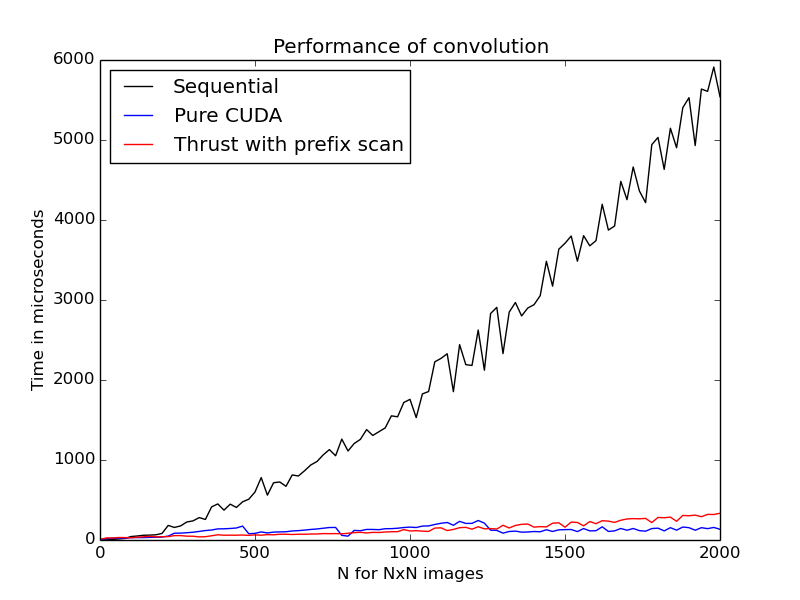
\includegraphics[scale=0.4]{imgs/performance.png}
    
    \end{figure}
\end{frame}

\begin{frame}{For each Implementation - Analysis}
  \begin{figure}
    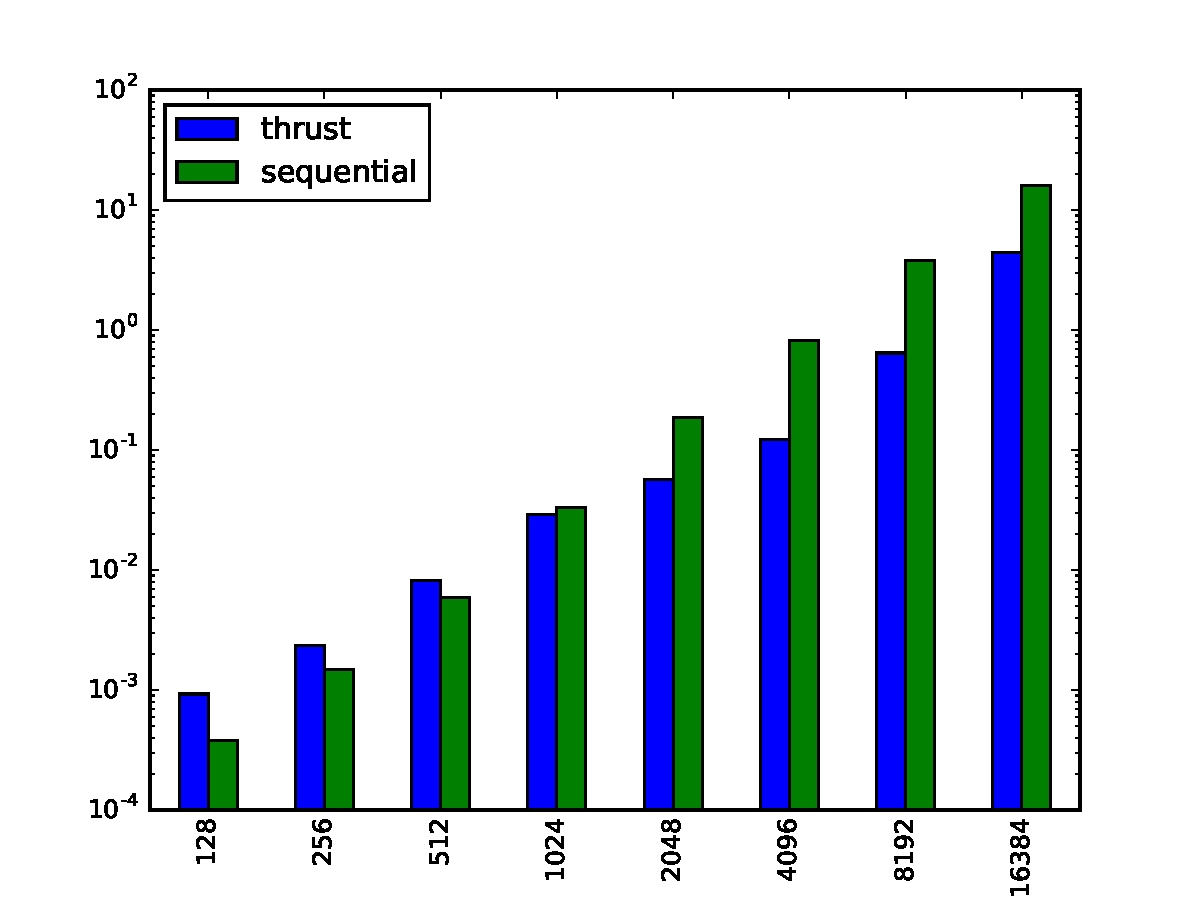
\includegraphics[scale=0.4]{imgs/thrust_vs_sequential_total.pdf} 
  \end{figure}
\end{frame} 

\begin{frame}{A closer look}
  \begin{figure}
    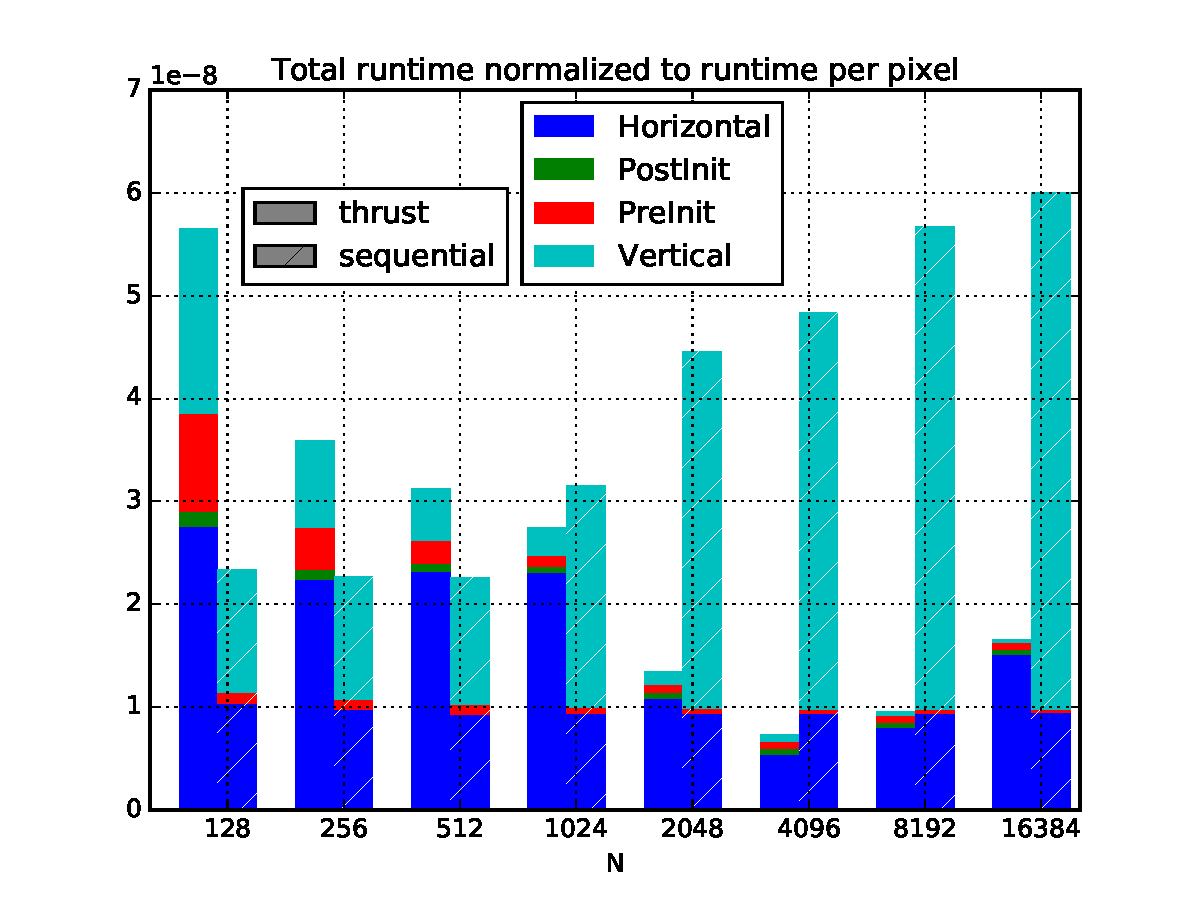
\includegraphics[scale=0.4]{imgs/thrust_vs_sequential_normalized.pdf} 
  \end{figure}
\end{frame} 


\section{Conclusion} 
\frame{\frametitle{Conclusion}
ToDo: Compare to FIR and FFT.
Explore blocked parallelism.
Hide data transfers.
}

%\begin{frame}[t, allowframebreaks]
\begin{frame}[t]
  \frametitle{References}
  \bibliographystyle{amsalpha}
  \bibliography{doc.bib}
\end{frame}

\end{document}
